\section{Interface Utilisateur}
\label{sec:interface}

\subsection{Une approche centrée utilisateur}
Depuis le début du projet Datapic, l’approche a été technique et statistique avant d’être métier. En plus d’améliorer la précision du prédicteur, l’un des principaux objectifs de cette PR était de mieux intégrer les besoins du Pic’Asso, et de \textbf{passer d’un proof of concept technique à un produit} utilisable par les équipes.

“Il faut développer l’interface et les prédictions pour qu’elles aient plus de sens pour les responsables”

Le but était de développer une couche applicative, qui puisse rendre les résultats du modèle statistique accessibles et facilement interprétables par les utilisateurs. Respecter une conception centrée sur l'utilisateur était une priorité dans la construction de cette partie, plus importante que ses performances : il faut que l'utilisateur puisse obtenir rapidement les informations dont il a besoin, et qu'il soit satisfait par les fonctionnalités proposée.

La première étape était donc de rassembler des idées de fonctionnalités exploitant les données du modèle statistique. Le besoin qui est apparu en premier pour les équipes du Pic'Asso se rapproche de celui d'un ERP (Entreprise Resource Planning): gestion du stock, assistance à la création des commandes, suivi de l'inventaire... Les fonctionnalités sont détaillées dans la partie \ref{subsec:ui_features}.

\subsection{L'interface existante}
\label{subsec:current_ui}

Le travail réalisé précédemment sur le projet Datapic a abouti au développement d'une application web, qui permet d'afficher les prédictions sur un intervalle de temps donné. Bien qu'efficace pour afficher les résultats du modèle statistique qui avait été développé, l'application n'était pas utilisable en soi par les équipes du Pic’Asso car elle donnait des prédictions sur les catégories et non sur les articles.

\begin{figure}[ht]
    \centering
    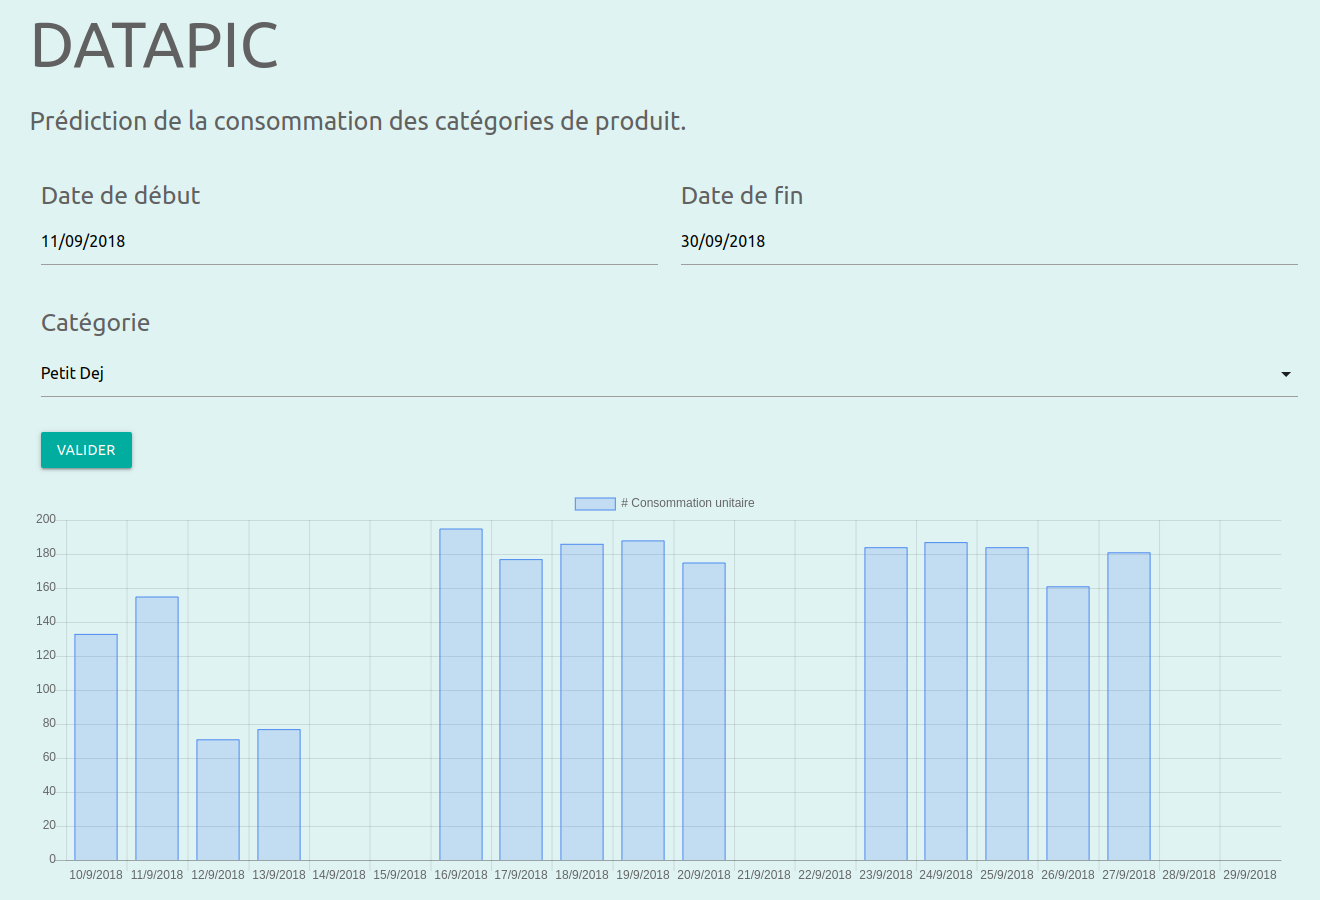
\includegraphics[width=0.9\textwidth]{figures/4_interface/flask.png}
    \caption{L'application web développée auparavant}
    \label{fig:flask_interface}
\end{figure}


\subsection{Les choix techniques réalisés}
\label{subsec:ui_techs}

La priorité a été donnée à la simplicité dans la stack technique. Dans la continuité de l’interface précédemment développée, le choix du langage Python était évident pour garder la cohérence avec le reste du projet, et faciliter l’intégration des différents éléments entre eux. Contrairement à l’interface existante développée avec Python et Flask, nous avons choisi d’utiliser le framework Django pour sa simplicité et rapidité de développement :
\begin{itemize}
    \item Il permet une grande évolutivité afin d’ajouter plus tard des fonctionnalités au projet, en altérant un minimum le code existant ─ notamment grâce à l’architecture Modèle-Template-Vue (implémentation de MVC). C’est un point important car l’application sera amenée à évoluer avec les retours des équipes d'approvisionnement du Pic'Asso.
    \item En plus d’être un standard, le framework Django est maîtrisé par plusieurs membres de l’équipe, et est cohérent avec la stack utilisée au Pic’Asso.
    \item De plus il permet de développer à la fois le front-end et le back-end facilement.
\end{itemize}


L'interfaçage avec la base de données Arango n’est pas disponible nativement dans le framework, mais l’intégration a été facile grâce au package \code{python-arango} déjà utilisé pour le modèle.

Étant donné que l’application sera utilisée par un nombre restreint d’utilisateurs, il n’y a pas de problématiques de scalabilité et de besoins élevés en performance. Avec le système de templates de django, les pages sont générées côté serveur, mais cela n’empêche pas d’avoir des temps de chargement rapides, le cache de django étant très efficace. Les seuls composants générés dynamiquement côté client sont les graphes : avec l'outil \code{chart.js}.

\subsection{Fonctionnalités}
\label{subsec:ui_features}

Le sujet laisse la porte ouverte au développement de nombreuses fonctionnalités, car un modèle de prédiction efficace ouvre beaucoup de perspectives. Les premières discussions ont fait émerger un axe qui était central dans le développement de l'interface : l'assistance à la gestion des stocks. La plupart de fonctionnalités évoquées se rapprochent en fait de celles d'un ERP :

\begin{itemize}
    \item Réalisation assistée de commandes en fonction de la demande à venir et des stocks restants
    \item OCR pour les factures et les tarifs avec ajout automatique aux stocks et aux descriptif produit
    \item Liste et Détail des Fournisseurs et Producteurs (compagnie, nom, mail, tel, produits proposés, actions en cours...)
    \item Calcul de pertes (e.g. portion du fût perdu)
    \item Aide à la décision au niveau des commandes (actions fournisseurs / promotions)
    \item Visualisation de l’évolution des stocks (graphiques)
    \item Assistance à l'inventaire manuel
    \item Statistiques sur les ventes en CA, quantité, sur la durée de vie d’un fût... pour améliorer la logistique et mieux évaluer le succès de certains produits
    \item Statistiques sur la fréquentation
    \item Comparaison entre différentes périodes
\end{itemize}

L'ensemble des fonctionnalités implémentées est détaillé dans la documentation de l'interface sur le GitLab du projet DataPic. Voici l'état de développement des fonctionnalités principales :


\begin{table}[H]
    \centering
    \begin{tabular}{c|c}
        \hline
        Fonctionnalité                             & État \\
        \hline
        Architecture django \& routes              & Implémenté \\
        Affichage de la liste des produits         & Implémenté \\
        Affichage des détails d'un produit         & Implémenté \\
        Affichage des graphes des ventes           & Implémenté \\
        Calcul du stock restant d'un produit       & Implémenté \\
        Estimation de la durée de vie restante     & À améliorer \\
        Outil d'aide à l'inventaire                & À implémenter \\
        Assistance à la réalisation de commandes   & À implémenter \\
    \end{tabular}
    \caption{État du développement des fonctionnalités principales de l'interface}
    \label{tab:tab_fonctionnalités}
\end{table}